\documentclass[letterpaper]{article}

\usepackage{graphicx}
\usepackage{alltt}
\usepackage{float}

\DeclareGraphicsExtensions{.png}

\begin{document}

\author{Christopher Sasarak}
\title{Summary of Min Refactor}
\maketitle

\section*{How to Read this Document}

I will refer to the version of Min with the old events system as 'Min Classic'.
When I make reference to just Min, I am referring to the latest version in the
master branch and on http://saskatoon.cs.rit.edu/min.
You can see Min Classic by checking out the tag \verb+min_classic+ from the git
repository: \begin{verbatim} git checkout min_classic \end{verbatim} You can
checkout Min by using \begin{verbatim} git checkout master \end{verbatim}

I will also make reference to \textbf{editing modes} in both Min and Min Classic.
When I refer to an editing mode, I am referring to a state of the editor that is
visible by the user. For example, when the pen icon is shaded and the user can
draw/type symbols into the system I will refer to it as 'pen mode'.

\section*{Event System Descriptions}

\subsection*{Min Classic Event System} 
Most of the events used by Min Classic are stored in the \verb+Editor.Events.js+ file. 
The listeners for buttons are bound in \verb+Editor.setup_events+ and will not
change for the life of the running Min instance. These button events are moved
but are mostly unaltered between Min Classic and the refactored
version. Likewise, events related to \verb+keypress+ events are largely the
same in Min; aside from being bound in different places/times. The Hammer events
used for the multi-touch pinch-to-resize functionality are moved to a different
file, but largely unchanged.

The majority of Min Classic's behavior are bound to the \verb+equation_canvas+
div; where a div is just a 'division' of the document and is used to group multiple
HTML elements together. Those event handlers are named as follows:
\verb+Editor.onMouseDown+, \verb+Editor.onMouseMove+,
\verb+Editor.onMouseUp+, \verb+Editor.onDoubleClick+. These events are
responsible for drawing, selecting segments, moving segments, and resizing
segments, i.e. the vast majority of user interaction. 

In Min Classic, the state was maintained by having a global
object which maps states to constant integer literals (behaving like an enumeration in Java or C)
declared in \verb+Editor.Events.js+ called \verb+EditorState+.
As the system runs, the currently running state is maintained in the variable
Editor.state. Editor states do no necessarily correspond directly to modes, it
is possible for an editor mode to make use of multiple editor states. 

Because the Javascript events bound to the \verb+equation_canvas+ div are never
changed for the life of a Min session, they each contain a switch statement
which determines which of their possible behaviors to use. The case to use is
selected by the current Editor state.

One weakness of this system is that the programmer must make sure that she sets
the Editor.state variable appropriately when adding new functionality. Doing
this incorrectly means that Min Classic could exhibit behavior appropriate for
other states. Additionally, it can be very difficult to locate where bugs are.
For example, to fix a bug in draw mode, the programmer might also have to look
at the code pertaining to the other modes rather than just draw mode.  

\subsection*{New Event System}

In order to address some of the shortcomings of the old event system, the DPRL
designed and implemented a new one which tries to handle the complexity of Min
with a (hopefully) cleaner approach. The main goals of this refactoring were:

\begin{enumerate}
    \item To make Min easier to hack for newcomers.  
    \item To make it easier to identify where bugs are caused.
    \item To separate concerns in the event system.
    \item To eliminate the use of EditorState as much as possible.
\end{enumerate}

The new Min event system is designed under the idea that the functionality of
Min can be separated into several discrete modes: \textbf{Draw Mode},
\textbf{Stroke Selection Mode}, and \textbf{Rectangle Selection Mode}. By
keeping track of the modes, we know which functionality should be active and
which should not be. Thus when the user switches from one mode to another, we know
exactly which mouse events are bound and which ones are not. To incorporate
additional dependent functionality one event can unbind and bind other events.
For example, in either of the selection modes, the
code for moving segments should only be bound/active when there are segments
already selected. In this case, the mouseDown event binds the mouseMove event
after it has determined that the user has just clicked a segment. The
relationships and prototype chain of this new system are shown visually in
Figure \ref{fig:modes}. Note that the selection modes share functionality and
that all events have EditorMode at the top of their prototype chain.

Important files in the new setup are:
\begin{description}
    \item[Editor.PermEvents.js] This file contains events which are bound when
        Min starts and then left alone. This is where the events attached to the
        buttons on the top-bar are located.
    \item[Editor.EditorMode.js] This file contains code that will be used by
        all EditorModes. All *Mode style objects have an instance of this object
        at the top of their prototype chain.
    \item[Editor.DrawMode.js] This file contains the objects that are used for
        behavior that is active in DrawMode, such as the typing tool and the
        drawing tool.
    \item[Editor.SelectionMode.js] Both rectangle and stroke selection mode
        contain a lot of shared behavior. They do movement and resizes in
        exactly the same way, the only difference is how they select strokes.
        Events common to both is in this file. This is part of the prototype
        chain for selection modes.
    \item[Editor.RectangleSelectionMode.js] This contains code specific to
        rectangle selection. When a segment is selected, SelectionMode takes
        over.
    \item[Editor.StrokeSelectionMode.js] This contains code specific to stroke
        selection. When a segment is selected, the events in SelectionMode take
        over.
\end{description}

\begin{figure}[h]
    \begin{center}
        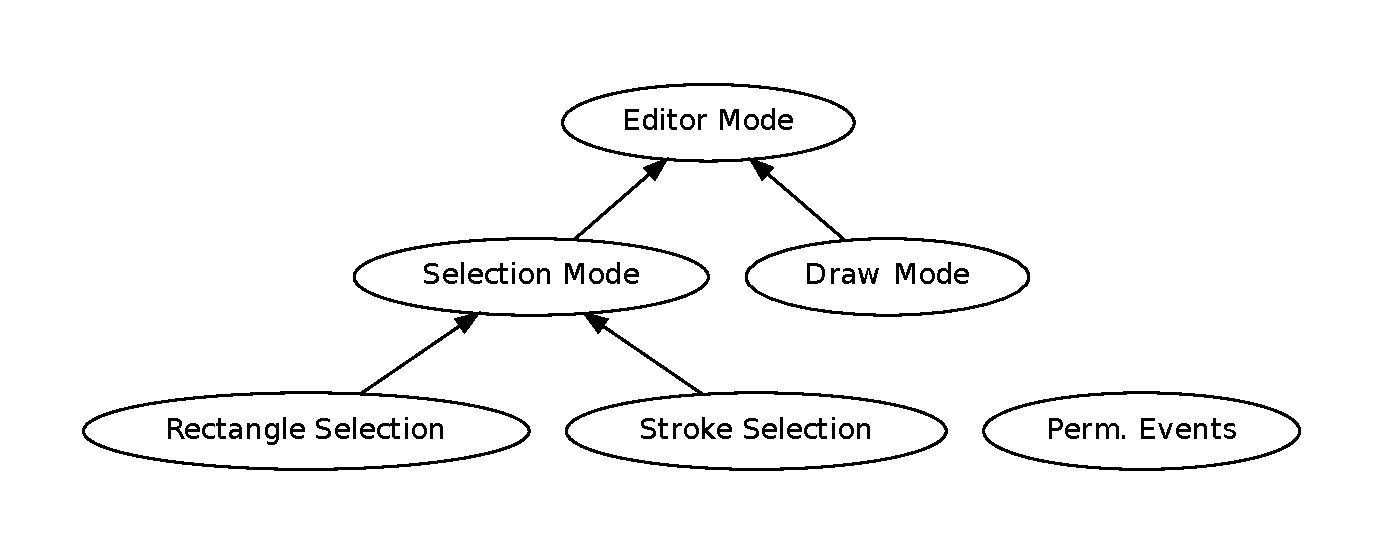
\includegraphics[width=\textwidth]{mode_diagram}
    \end{center}
    \caption{The prototype chain of the new editor modes}
    \label{fig:modes}
\end{figure}

\subsection*{Other Changes}

One final change that I made during refactoring was the addition of the
Modernizr library. Modernizr is a BSD/MIT licensed library which runs when the
document loads and queries the browser for its capabilities. Currently I only use it to
check for the touch-screen interface. Originally, we just checked the user-agent
string to see if it had the 'iPad' in it. Modernizer provides a consistent
interface for checking for touch-screen functionality under a Free Software
license.

\subsection*{Front End to Back End Flow}
\begin{figure}[H]
    \begin{center}
        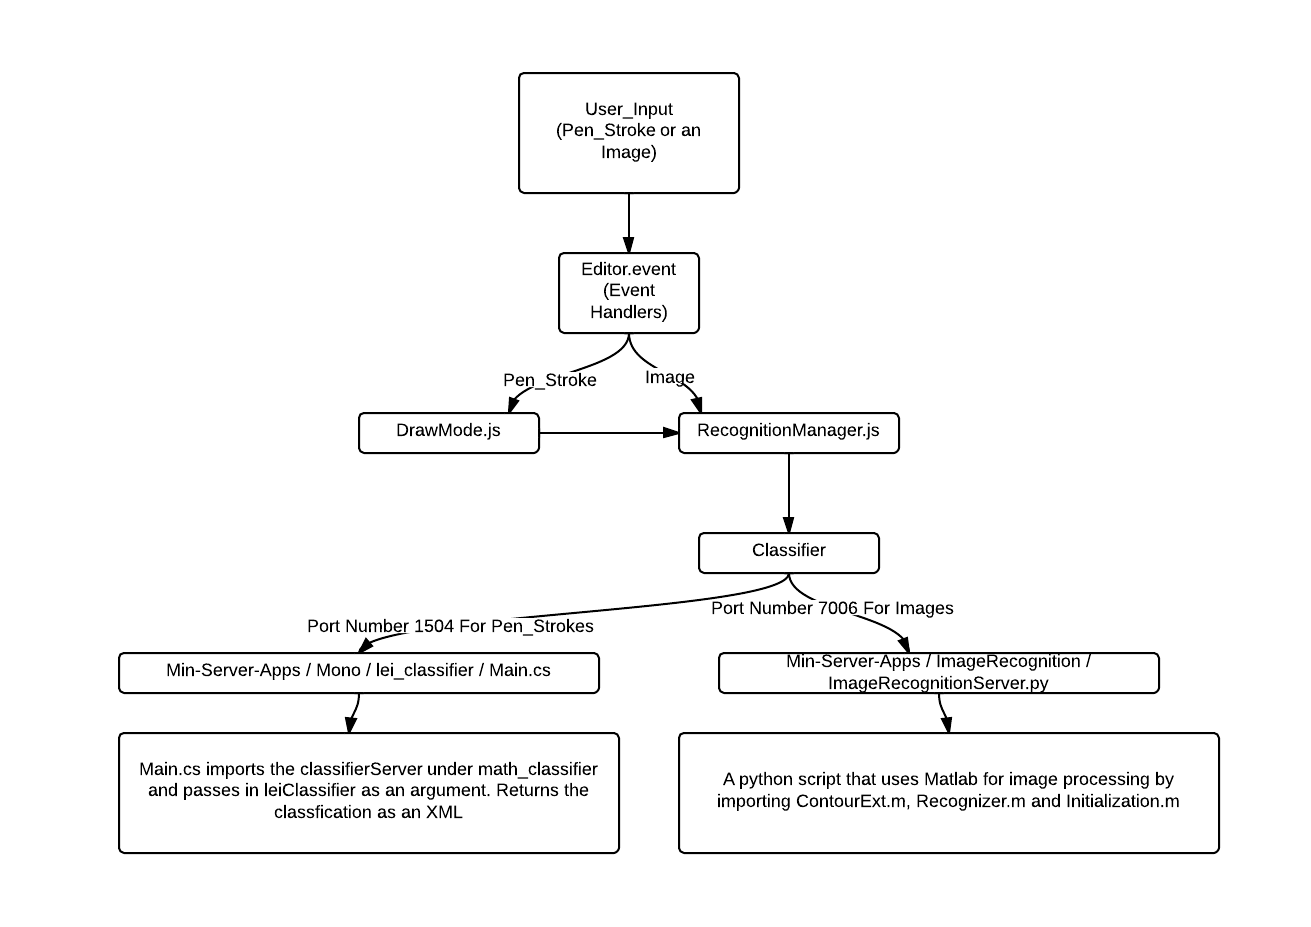
\includegraphics[width=\textwidth]{FrontToBackEndFlow.png}
    \end{center}
    \caption{The flow from Front-End to Back-End processes}
    \label{fig:frontToBack}
\end{figure}

The Min event system accepts three types of input: keyboard inputs, pen strokes, and
image files. Each type of input will fire a different function. Keyboard input does
not require recognition so nothing further is done at this point for it. Pen strokes
will activate \verb+DrawMode+ which records the position of the strokes. Image files
will trigger \verb+onImageLoad+.

From here, pen strokes and images will both be sent to the \verb+RecognitionManager+.
The \verb+RecognitionManager+ enqueues all of the inputs and then calls \verb+Classifier+
to get a classification for each. Pen strokes and images are sent to different functions
for separate classification.

Pen strokes are sent through port 1504 to the \verb+Main+ class of \verb+Mono/lei_classifier+.
This will make a call to a \verb+ClassifierServer+ which uses the \verb+LeiClassifier+ to
classify the pen strokes. The results are returned as an XML.

Images are sent through port 7006 to the \verb+ImageRecognitionServer+. This server will
call on Matlab scripts to do the image processing. Matlab will segment the image and then
classify each separate part of the image. These results are converted to an XML and returned.

The front end of the system recieves the XML of the classified symbols. \verb+Classifier+
processes the XML and creates recognition which is put in the \verb+RecognitionManager+'s
result table. Then the \verb+RenderManager+ renders the canvas, displaying the recognized
symbols.


\subsection*{TODO}
Here are some things that I would like to see happen that are closely related to
the event system refactoring.

\begin{description}
    \item[Remove references to EditorState] Currently there are still references
        to EditorState in the events system. I left this in place because there
        are a few subsystems, like RenderManager, that rely on EditorState. So
        while none of the systems that I have changed (to my knowledge) use
        Editor.state to make decisions, changes to EditorState were left in
        place for the sake of other systems I was not working with at the time.
        Ideally we could completely eliminate references to EditorState and
        Editor.state throughout the system.
    \item[Remove Legacy Code] There is likely some code in the Min events' system
        that could have been removed, but that I missed. 
    \item[Consolidate Keypress Code] Currently we have a couple different
        functions (mapCanvasBackspace, onKeyPress) that can be called to handle key-presses. We should
        consolidate these event handlers where possible and move functionality
        to more appropriate places if possible. It might also be worth
        investigating if mapCanvasBackspace is still necessary, or if there's a
        better way to do it.
    \item[Replace *.proxy Calls with .bind] This is a fairly trivial change. I
        make heavy use of jQuery's .proxy method to make sure that when an event
        is called, the special 'this' reference refers to the EditorMode object
        that is currently active. By default, in Javascript and event handler
        function's 'this' reference points to the DOM object which the event was
        fired on. I wanted to use 'this' the way that Java might so that I could
        store mode-specific state in the mode objects rather than as a global. I
        used .proxy, not knowing that modern browsers have a function called
        bind which does the same thing. We should use this method where possible
        since it will likely be a bit faster. See Editor.SelectionMode.js and
        its constructor for an example of both.
    \item[Further Separate Event Functions into Modes] It might be
        possible to further separate concerns in some of the larger functions of
        the *Mode objects even further. 
\end{description}

\section*{Further Potential Refactors}

\begin{description}
    \item[Disable Image Upload Appropriately] Currently it is possible to click the image
        upload button when in either rectangle or stroke select mode. This is
        inconsistent with behavior that we already have which disables
        drawing/typing tools in selection mode. The button should probably turn
        itself off when in either of the selection modes or clicking it in the
        selection modes should automatically switch the user back into draw
        mode.
    \item[Remove Collision Manager] The collision manager is currently used to
        determine where on the equation\_canvas the user has clicked. For
        example, if you look at any of the onDown base functions you will see a
        call to the CollisionManager somewhere towards the beginning. This is
        not an optimal use of resources, since rather than detecting if a
        click happened on a segment, you could just bind the onclick event to
        the segments themselves and let the browser do the work rather than
        forcing Javascript code to do it. CollisionManager may still have some
        use in that it helps choose which segment to select when multiple
        segments are stacked on top of each other on the canvas. However,
        dynamicaly setting the z-index CSS style attribute might be a better
        choice to get this behavior. Ultimately it would make the system much
        simpler and likely more extensible if we can eliminate the
        CollisionManager.
    \item[Remove RenderManager] Earlier versions of Min made use of a 'canvas'
        element. Note that this is the \emph{type} of element, not the id of the
        element. The problem with this is that we must manually re-render (via
        RenderManager) when we want to update where our segments are on the
        canvas. Not only that, but we have to re-render for \emph{every} frame
        when we are animating moving or resizing segments. 
        
        In the meantime a technology called Scalable Vector Graphics (SVG) has
        gotten widespread and mature support in modern browsers. This is a
        better choice to use wherever possible because changes to SVG objects
        (even animations) can be performed just by changing attributes on SVG
        HTML elements. An advantage is that rendering is performed by the
        browser, which (usually) has built in support for SVG. If we can change
        all of Min to use and properly update SVG objects, we can hopefully
        eliminate the RenderManager and be left with a system that will be
        significantly  more responsive.
    \item[Remove Editor.* Prefixes] Many files and objects have an Editor.*
        prefix. While this is reasonable for global variables being stored on
        the Editor object, in my opinion mostly just makes the names of things longer
        without adding much extra information. Hint: With a few well-written
        \verb+sed+ invocations this should be much easier.
    \item[Streamline the Classifier] The objects and methods related to
        classification to be difficult to navigate. If the Classifier and its
        related code can be made more transparent, the classification code will
        be easier to maintain.
    \item[Remove segment\_id and set\_id] During editing, the
        user can combine and separate strokes; such as the horizontal and
        vertical strokes in a '+'. In one interpretation, there is a single
        symbol composed of two separate strokes, and in the other both of the
        strokes are their own symbol. To keep track of which segments are which
        and how they are grouped Min assigned each segment both a
        \verb+segment_id+ and a \verb+set_id+. Every segment should have its own
        unique (for that particular instance of of Min) \verb+segment_id+. If multiple segments are in the
        same symbol, in addition to to their \verb+segment_id+ they will share
        a \verb+set_id+. The problem is that maintaining these numbers properly
        can be difficult: numerous bugs have popped up because set or segment
        ids get changed to something wrong in the course of Min's run. Combine
        that with the fact that the back-end server for image upload needs to
        have some knowledge of available segment/set ids and it becomes even
        more difficult. I think a better approach would be to combine strokes on
        the canvas using something called the \emph{composite pattern}.
        Wikipedia provides a good overview of composite pattern, but a quick
        summary is that the composite pattern is a way to give singular objects
        and multiple objects the same interface, so they can be used
        interchangeably. This makes the segment/set issue simpler because it
        makes the groupings of the strokes intrinsic in their DOM structure.  % reword?
    \item[Min only presents 56 different symbol classes] Though we have
         classifiers that support more than this, Min only presents 56 different
         classes to the user. We should increase this as users sometimes ask why a
         particular letter or symbol is not available. Look at
         \verb+example_tree_icdar.xml+ as a starting point.
       
\end{description}

\section*{Tips}
\begin{description}
    \item[Learn about prototypal inheritance] The majority of OOP languages are
        based on classes which are then instantiated into objects which actually
        encapsulate data and perform computations. Javascript is not one of
        these languages. Javascript makes use of prototypal inheritance. In this
        situation objects are created directly, and new objects are cloned from
        these existing ones. In the new Min events' system, I make heavy use of
        this fact. You should study what prototypal inheritance is and get a
        sense for how Javascript does OOP.
    \item[Learn to use 'grep'] grep is a command-line tool for searching files
        on Unix and Unix-like systems. It allows you to search multiple files
        for either a string or a regex. Learn to use it, the computer is better
        than you at finding things.
    \item[Mozilla Developer Network] The MDN is useful for virtually anything
        having to do with designing a website. It is comprehensive and can
        really help if you get stuck.
    \item[Unix Tutorials] I have found these tutorials helpful in making my work
        more pleasant: http://www.grymoire.com/Unix/ 
        In particular I make fairly heavy use of sed in my day-to-day
        development. It makes trivial, but tedious changes to code much
        simpler.
    \item[Git] Git is a tool with a steep learning curve that can also make your
        life \emph{much} easier if you learn to use it well. I recommend these
        sites for help:\\ 
        http://try.github.io - An interactive tutorial for learning to use
        Git.\\
        http://gitready.com/ - Not so much a tutorial as a series of tips for
        doing cool things with Git.\\
        http://git-scm.com/book - This is a book for Git which is available for
        free online. \\
        'git help' - This is a way to access the Git manpages. 
        Just run \verb+git help+.
\end{description}

\end{document}
